\documentclass[1p]{elsarticle_modified}
%\bibliographystyle{elsarticle-num}

%\usepackage[colorlinks]{hyperref}
%\usepackage{abbrmath_seonhwa} %\Abb, \Ascr, \Acal ,\Abf, \Afrak
\usepackage{amsfonts}
\usepackage{amssymb}
\usepackage{amsmath}
\usepackage{amsthm}
\usepackage{scalefnt}
\usepackage{amsbsy}
\usepackage{kotex}
\usepackage{caption}
\usepackage{subfig}
\usepackage{color}
\usepackage{graphicx}
\usepackage{xcolor} %% white, black, red, green, blue, cyan, magenta, yellow
\usepackage{float}
\usepackage{setspace}
\usepackage{hyperref}

\usepackage{tikz}
\usetikzlibrary{arrows}

\usepackage{multirow}
\usepackage{array} % fixed length table
\usepackage{hhline}

%%%%%%%%%%%%%%%%%%%%%
\makeatletter
\renewcommand*\env@matrix[1][\arraystretch]{%
	\edef\arraystretch{#1}%
	\hskip -\arraycolsep
	\let\@ifnextchar\new@ifnextchar
	\array{*\c@MaxMatrixCols c}}
\makeatother %https://tex.stackexchange.com/questions/14071/how-can-i-increase-the-line-spacing-in-a-matrix
%%%%%%%%%%%%%%%

\usepackage[normalem]{ulem}

\newcommand{\msout}[1]{\ifmmode\text{\sout{\ensuremath{#1}}}\else\sout{#1}\fi}
%SOURCE: \msout is \stkout macro in https://tex.stackexchange.com/questions/20609/strikeout-in-math-mode

\newcommand{\cancel}[1]{
	\ifmmode
	{\color{red}\msout{#1}}
	\else
	{\color{red}\sout{#1}}
	\fi
}

\newcommand{\add}[1]{
	{\color{blue}\uwave{#1}}
}

\newcommand{\replace}[2]{
	\ifmmode
	{\color{red}\msout{#1}}{\color{blue}\uwave{#2}}
	\else
	{\color{red}\sout{#1}}{\color{blue}\uwave{#2}}
	\fi
}

\newcommand{\Sol}{\mathcal{S}} %segment
\newcommand{\D}{D} %diagram
\newcommand{\A}{\mathcal{A}} %arc


%%%%%%%%%%%%%%%%%%%%%%%%%%%%%5 test

\def\sl{\operatorname{\textup{SL}}(2,\Cbb)}
\def\psl{\operatorname{\textup{PSL}}(2,\Cbb)}
\def\quan{\mkern 1mu \triangleright \mkern 1mu}

\theoremstyle{definition}
\newtheorem{thm}{Theorem}[section]
\newtheorem{prop}[thm]{Proposition}
\newtheorem{lem}[thm]{Lemma}
\newtheorem{ques}[thm]{Question}
\newtheorem{cor}[thm]{Corollary}
\newtheorem{defn}[thm]{Definition}
\newtheorem{exam}[thm]{Example}
\newtheorem{rmk}[thm]{Remark}
\newtheorem{alg}[thm]{Algorithm}

\newcommand{\I}{\sqrt{-1}}
\begin{document}

%\begin{frontmatter}
%
%\title{Boundary parabolic representations of knots up to 8 crossings}
%
%%% Group authors per affiliation:
%\author{Yunhi Cho} 
%\address{Department of Mathematics, University of Seoul, Seoul, Korea}
%\ead{yhcho@uos.ac.kr}
%
%
%\author{Seonhwa Kim} %\fnref{s_kim}}
%\address{Center for Geometry and Physics, Institute for Basic Science, Pohang, 37673, Korea}
%\ead{ryeona17@ibs.re.kr}
%
%\author{Hyuk Kim}
%\address{Department of Mathematical Sciences, Seoul National University, Seoul 08826, Korea}
%\ead{hyukkim@snu.ac.kr}
%
%\author{Seokbeom Yoon}
%\address{Department of Mathematical Sciences, Seoul National University, Seoul, 08826,  Korea}
%\ead{sbyoon15@snu.ac.kr}
%
%\begin{abstract}
%We find all boundary parabolic representation of knots up to 8 crossings.
%
%\end{abstract}
%\begin{keyword}
%    \MSC[2010] 57M25 
%\end{keyword}
%
%\end{frontmatter}

%\linenumbers
%\tableofcontents
%
\newcommand\colored[1]{\textcolor{white}{\rule[-0.35ex]{0.8em}{1.4ex}}\kern-0.8em\color{red} #1}%
%\newcommand\colored[1]{\textcolor{white}{ #1}\kern-2.17ex	\textcolor{white}{ #1}\kern-1.81ex	\textcolor{white}{ #1}\kern-2.15ex\color{red}#1	}

{\Large $\underline{12n_{0396}~(K12n_{0396})}$}

\setlength{\tabcolsep}{10pt}
\renewcommand{\arraystretch}{1.6}
\vspace{1cm}\begin{tabular}{m{100pt}>{\centering\arraybackslash}m{274pt}}
\multirow{5}{120pt}{
	\centering
	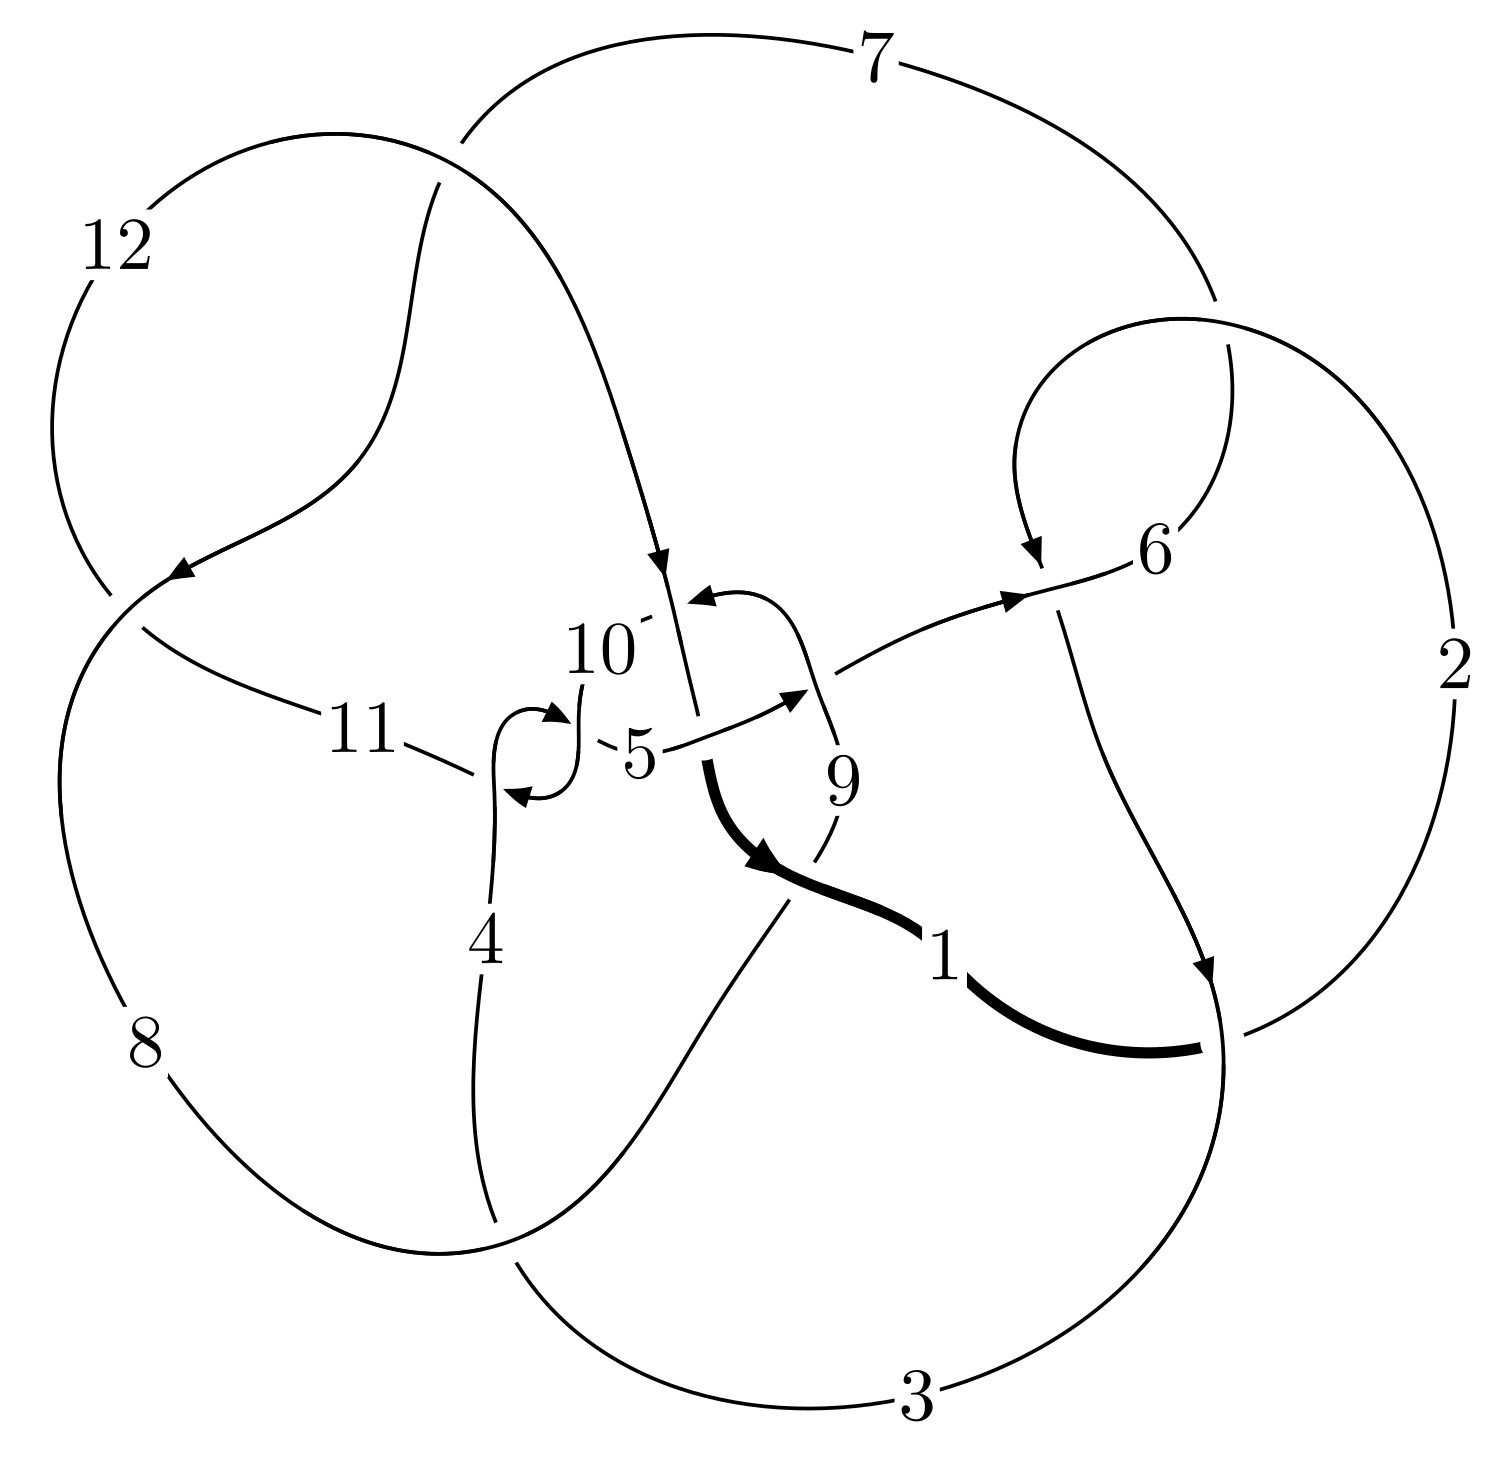
\includegraphics[width=112pt]{../../../GIT/diagram.site/Diagrams/png/2485_12n_0396.png}\\
\ \ \ A knot diagram\footnotemark}&
\allowdisplaybreaks
\textbf{Linearized knot diagam} \\
\cline{2-2}
 &
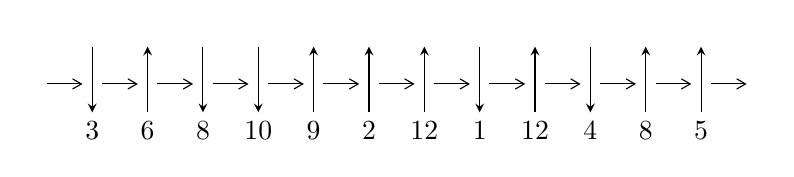
\begin{tikzpicture}[x=20pt, y=17pt]
	% nodes
	\node (C0) at (0, 0) {};
	\node (C1) at (1, 0) {};
	\node (C1U) at (1, +1) {};
	\node (C1D) at (1, -1) {3};

	\node (C2) at (2, 0) {};
	\node (C2U) at (2, +1) {};
	\node (C2D) at (2, -1) {6};

	\node (C3) at (3, 0) {};
	\node (C3U) at (3, +1) {};
	\node (C3D) at (3, -1) {8};

	\node (C4) at (4, 0) {};
	\node (C4U) at (4, +1) {};
	\node (C4D) at (4, -1) {10};

	\node (C5) at (5, 0) {};
	\node (C5U) at (5, +1) {};
	\node (C5D) at (5, -1) {9};

	\node (C6) at (6, 0) {};
	\node (C6U) at (6, +1) {};
	\node (C6D) at (6, -1) {2};

	\node (C7) at (7, 0) {};
	\node (C7U) at (7, +1) {};
	\node (C7D) at (7, -1) {12};

	\node (C8) at (8, 0) {};
	\node (C8U) at (8, +1) {};
	\node (C8D) at (8, -1) {1};

	\node (C9) at (9, 0) {};
	\node (C9U) at (9, +1) {};
	\node (C9D) at (9, -1) {12};

	\node (C10) at (10, 0) {};
	\node (C10U) at (10, +1) {};
	\node (C10D) at (10, -1) {4};

	\node (C11) at (11, 0) {};
	\node (C11U) at (11, +1) {};
	\node (C11D) at (11, -1) {8};

	\node (C12) at (12, 0) {};
	\node (C12U) at (12, +1) {};
	\node (C12D) at (12, -1) {5};
	\node (C13) at (13, 0) {};

	% arrows
	\draw[->,>={angle 60}]
	(C0) edge (C1) (C1) edge (C2) (C2) edge (C3) (C3) edge (C4) (C4) edge (C5) (C5) edge (C6) (C6) edge (C7) (C7) edge (C8) (C8) edge (C9) (C9) edge (C10) (C10) edge (C11) (C11) edge (C12) (C12) edge (C13) ;	\draw[->,>=stealth]
	(C1U) edge (C1D) (C2D) edge (C2U) (C3U) edge (C3D) (C4U) edge (C4D) (C5D) edge (C5U) (C6D) edge (C6U) (C7D) edge (C7U) (C8U) edge (C8D) (C9D) edge (C9U) (C10U) edge (C10D) (C11D) edge (C11U) (C12D) edge (C12U) ;
	\end{tikzpicture} \\
\hhline{~~} \\& 
\textbf{Solving Sequence} \\ \cline{2-2} 
 &
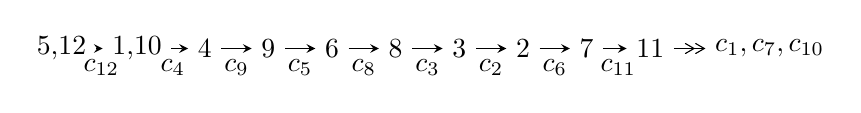
\begin{tikzpicture}[x=23pt, y=7pt]
	% node
	\node (A0) at (-1/8, 0) {5,12};
	\node (A1) at (17/16, 0) {1,10};
	\node (A2) at (17/8, 0) {4};
	\node (A3) at (25/8, 0) {9};
	\node (A4) at (33/8, 0) {6};
	\node (A5) at (41/8, 0) {8};
	\node (A6) at (49/8, 0) {3};
	\node (A7) at (57/8, 0) {2};
	\node (A8) at (65/8, 0) {7};
	\node (A9) at (73/8, 0) {11};
	\node (C1) at (1/2, -1) {$c_{12}$};
	\node (C2) at (13/8, -1) {$c_{4}$};
	\node (C3) at (21/8, -1) {$c_{9}$};
	\node (C4) at (29/8, -1) {$c_{5}$};
	\node (C5) at (37/8, -1) {$c_{8}$};
	\node (C6) at (45/8, -1) {$c_{3}$};
	\node (C7) at (53/8, -1) {$c_{2}$};
	\node (C8) at (61/8, -1) {$c_{6}$};
	\node (C9) at (69/8, -1) {$c_{11}$};
	\node (A10) at (11, 0) {$c_{1},c_{7},c_{10}$};

	% edge
	\draw[->,>=stealth]	
	(A0) edge (A1) (A1) edge (A2) (A2) edge (A3) (A3) edge (A4) (A4) edge (A5) (A5) edge (A6) (A6) edge (A7) (A7) edge (A8) (A8) edge (A9) ;
	\draw[->>,>={angle 60}]	
	(A9) edge (A10);
\end{tikzpicture} \\ 

\end{tabular} \\

\footnotetext{
The image of knot diagram is generated by the software ``\textbf{Draw programme}" developed by Andrew Bartholomew(\url{http://www.layer8.co.uk/maths/draw/index.htm\#Running-draw}), where we modified some parts for our purpose(\url{https://github.com/CATsTAILs/LinksPainter}).
}\phantom \\ \newline 
\centering \textbf{Ideals for irreducible components\footnotemark of $X_{\text{par}}$} 
 
\begin{align*}
I^u_{1}&=\langle 
-2.96098\times10^{119} u^{60}-8.03566\times10^{119} u^{59}+\cdots+1.57498\times10^{117} b-7.94333\times10^{120},\\
\phantom{I^u_{1}}&\phantom{= \langle  }-4.40897\times10^{120} u^{60}-1.19687\times10^{121} u^{59}+\cdots+2.99247\times10^{118} a-1.18579\times10^{122},\\
\phantom{I^u_{1}}&\phantom{= \langle  }u^{61}+2 u^{60}+\cdots-76 u-19\rangle \\
I^u_{2}&=\langle 
-1.15866\times10^{17} u^{27}+2.41753\times10^{17} u^{26}+\cdots+7.07730\times10^{17} b+1.02954\times10^{18},\\
\phantom{I^u_{2}}&\phantom{= \langle  }3.01367\times10^{17} u^{27}+5.60690\times10^{16} u^{26}+\cdots+7.07730\times10^{17} a+1.80278\times10^{18},\;u^{28}- u^{27}+\cdots- u+1\rangle \\
\\
\end{align*}
\raggedright * 2 irreducible components of $\dim_{\mathbb{C}}=0$, with total 89 representations.\\
\footnotetext{All coefficients of polynomials are rational numbers. But the coefficients are sometimes approximated in decimal forms when there is not enough margin.}
\newpage
\renewcommand{\arraystretch}{1}
\centering \section*{I. $I^u_{1}= \langle -2.96\times10^{119} u^{60}-8.04\times10^{119} u^{59}+\cdots+1.57\times10^{117} b-7.94\times10^{120},\;-4.41\times10^{120} u^{60}-1.20\times10^{121} u^{59}+\cdots+2.99\times10^{118} a-1.19\times10^{122},\;u^{61}+2 u^{60}+\cdots-76 u-19 \rangle$}
\flushleft \textbf{(i) Arc colorings}\\
\begin{tabular}{m{7pt} m{180pt} m{7pt} m{180pt} }
\flushright $a_{5}=$&$\begin{pmatrix}0\\u\end{pmatrix}$ \\
\flushright $a_{12}=$&$\begin{pmatrix}1\\0\end{pmatrix}$ \\
\flushright $a_{1}=$&$\begin{pmatrix}1\\- u^2\end{pmatrix}$ \\
\flushright $a_{10}=$&$\begin{pmatrix}147.336 u^{60}+399.962 u^{59}+\cdots+21361.8 u+3962.58\\188.001 u^{60}+510.206 u^{59}+\cdots+27232.1 u+5043.44\end{pmatrix}$ \\
\flushright $a_{4}=$&$\begin{pmatrix}39.5209 u^{60}+107.101 u^{59}+\cdots+5741.11 u+1070.30\\182.349 u^{60}+493.732 u^{59}+\cdots+26284.5 u+4863.37\end{pmatrix}$ \\
\flushright $a_{9}=$&$\begin{pmatrix}-40.6653 u^{60}-110.244 u^{59}+\cdots-5870.31 u-1080.86\\188.001 u^{60}+510.206 u^{59}+\cdots+27232.1 u+5043.44\end{pmatrix}$ \\
\flushright $a_{6}=$&$\begin{pmatrix}76.4909 u^{60}+207.985 u^{59}+\cdots+11163.0 u+2075.69\\-219.319 u^{60}-594.616 u^{59}+\cdots-31704.4 u-5868.76\end{pmatrix}$ \\
\flushright $a_{8}=$&$\begin{pmatrix}126.765 u^{60}+344.336 u^{59}+\cdots+18391.7 u+3413.23\\103.129 u^{60}+279.972 u^{59}+\cdots+14952.3 u+2768.79\end{pmatrix}$ \\
\flushright $a_{3}=$&$\begin{pmatrix}43.5638 u^{60}+118.466 u^{59}+\cdots+6304.28 u+1174.55\\105.291 u^{60}+285.368 u^{59}+\cdots+15160.1 u+2799.38\end{pmatrix}$ \\
\flushright $a_{2}=$&$\begin{pmatrix}-28.7474 u^{60}-81.0140 u^{59}+\cdots-4637.56 u-879.035\\16.0573 u^{60}+44.4956 u^{59}+\cdots+2463.99 u+460.188\end{pmatrix}$ \\
\flushright $a_{7}=$&$\begin{pmatrix}-23.6360 u^{60}-64.3645 u^{59}+\cdots-3439.43 u-644.437\\-103.129 u^{60}-279.972 u^{59}+\cdots-14952.3 u-2768.79\end{pmatrix}$ \\
\flushright $a_{11}=$&$\begin{pmatrix}86.9161 u^{60}+235.789 u^{59}+\cdots+12531.9 u+2321.16\\223.821 u^{60}+605.501 u^{59}+\cdots+32142.9 u+5936.73\end{pmatrix}$\\&\end{tabular}
\flushleft \textbf{(ii) Obstruction class $= -1$}\\~\\
\flushleft \textbf{(iii) Cusp Shapes $= 21.9680 u^{60}+64.0290 u^{59}+\cdots+3263.11 u+632.215$}\\~\\
\newpage\renewcommand{\arraystretch}{1}
\flushleft \textbf{(iv) u-Polynomials at the component}\newline \\
\begin{tabular}{m{50pt}|m{274pt}}
Crossings & \hspace{64pt}u-Polynomials at each crossing \\
\hline $$\begin{aligned}c_{1}\end{aligned}$$&$\begin{aligned}
&u^{61}+25 u^{60}+\cdots+1370 u-1
\end{aligned}$\\
\hline $$\begin{aligned}c_{2},c_{6}\end{aligned}$$&$\begin{aligned}
&u^{61}- u^{60}+\cdots+34 u+1
\end{aligned}$\\
\hline $$\begin{aligned}c_{3}\end{aligned}$$&$\begin{aligned}
&u^{61}- u^{60}+\cdots+4446 u-457
\end{aligned}$\\
\hline $$\begin{aligned}c_{4},c_{10}\end{aligned}$$&$\begin{aligned}
&u^{61}- u^{60}+\cdots-1806 u-419
\end{aligned}$\\
\hline $$\begin{aligned}c_{5}\end{aligned}$$&$\begin{aligned}
&u^{61}-4 u^{60}+\cdots+1708 u-491
\end{aligned}$\\
\hline $$\begin{aligned}c_{7},c_{11}\end{aligned}$$&$\begin{aligned}
&u^{61}+u^{60}+\cdots+99546436 u-13493731
\end{aligned}$\\
\hline $$\begin{aligned}c_{8}\end{aligned}$$&$\begin{aligned}
&u^{61}+5 u^{60}+\cdots-3032 u-3995
\end{aligned}$\\
\hline $$\begin{aligned}c_{9}\end{aligned}$$&$\begin{aligned}
&u^{61}+14 u^{60}+\cdots-96977 u-34681
\end{aligned}$\\
\hline $$\begin{aligned}c_{12}\end{aligned}$$&$\begin{aligned}
&u^{61}-2 u^{60}+\cdots-76 u+19
\end{aligned}$\\
\hline
\end{tabular}\\~\\
\newpage\renewcommand{\arraystretch}{1}
\flushleft \textbf{(v) Riley Polynomials at the component}\newline \\
\begin{tabular}{m{50pt}|m{274pt}}
Crossings & \hspace{64pt}Riley Polynomials at each crossing \\
\hline $$\begin{aligned}c_{1}\end{aligned}$$&$\begin{aligned}
&y^{61}+37 y^{60}+\cdots+1971254 y-1
\end{aligned}$\\
\hline $$\begin{aligned}c_{2},c_{6}\end{aligned}$$&$\begin{aligned}
&y^{61}+25 y^{60}+\cdots+1370 y-1
\end{aligned}$\\
\hline $$\begin{aligned}c_{3}\end{aligned}$$&$\begin{aligned}
&y^{61}+121 y^{60}+\cdots+5985624 y-208849
\end{aligned}$\\
\hline $$\begin{aligned}c_{4},c_{10}\end{aligned}$$&$\begin{aligned}
&y^{61}+89 y^{60}+\cdots-560482 y-175561
\end{aligned}$\\
\hline $$\begin{aligned}c_{5}\end{aligned}$$&$\begin{aligned}
&y^{61}-16 y^{60}+\cdots-1860166 y-241081
\end{aligned}$\\
\hline $$\begin{aligned}c_{7},c_{11}\end{aligned}$$&$\begin{aligned}
&y^{61}-103 y^{60}+\cdots-592149097680014 y-182080776300361
\end{aligned}$\\
\hline $$\begin{aligned}c_{8}\end{aligned}$$&$\begin{aligned}
&y^{61}+15 y^{60}+\cdots-71386126 y-15960025
\end{aligned}$\\
\hline $$\begin{aligned}c_{9}\end{aligned}$$&$\begin{aligned}
&y^{61}-50 y^{60}+\cdots+15117817107 y-1202771761
\end{aligned}$\\
\hline $$\begin{aligned}c_{12}\end{aligned}$$&$\begin{aligned}
&y^{61}-8 y^{60}+\cdots+11324 y-361
\end{aligned}$\\
\hline
\end{tabular}\\~\\
\newpage\flushleft \textbf{(vi) Complex Volumes and Cusp Shapes}
$$\begin{array}{c|c|c}  
\text{Solutions to }I^u_{1}& \I (\text{vol} + \sqrt{-1}CS) & \text{Cusp shape}\\
 \hline 
\begin{aligned}
u &= \phantom{-}0.726966 + 0.679000 I \\
a &= -0.230767 - 0.059357 I \\
b &= -1.380190 + 0.112865 I\end{aligned}
 & -0.39695 + 7.20473 I & \phantom{-0.000000 } 0 \\ \hline\begin{aligned}
u &= \phantom{-}0.726966 - 0.679000 I \\
a &= -0.230767 + 0.059357 I \\
b &= -1.380190 - 0.112865 I\end{aligned}
 & -0.39695 - 7.20473 I & \phantom{-0.000000 } 0 \\ \hline\begin{aligned}
u &= -0.875047 + 0.392404 I \\
a &= -0.47290 + 2.04945 I \\
b &= -1.125280 - 0.174220 I\end{aligned}
 & \phantom{-}13.1897 - 5.2499 I & \phantom{-0.000000 } 0 \\ \hline\begin{aligned}
u &= -0.875047 - 0.392404 I \\
a &= -0.47290 - 2.04945 I \\
b &= -1.125280 + 0.174220 I\end{aligned}
 & \phantom{-}13.1897 + 5.2499 I & \phantom{-0.000000 } 0 \\ \hline\begin{aligned}
u &= -0.686697 + 0.668109 I \\
a &= -0.142029 - 0.279533 I \\
b &= -0.950069 - 0.505344 I\end{aligned}
 & \phantom{-}0.97517 - 2.05582 I & \phantom{-0.000000 } 0 \\ \hline\begin{aligned}
u &= -0.686697 - 0.668109 I \\
a &= -0.142029 + 0.279533 I \\
b &= -0.950069 + 0.505344 I\end{aligned}
 & \phantom{-}0.97517 + 2.05582 I & \phantom{-0.000000 } 0 \\ \hline\begin{aligned}
u &= -0.771408 + 0.558902 I \\
a &= \phantom{-}0.855387 + 0.424717 I \\
b &= -0.529958 + 0.377542 I\end{aligned}
 & \phantom{-}1.45455 - 2.20607 I & \phantom{-0.000000 } 0 \\ \hline\begin{aligned}
u &= -0.771408 - 0.558902 I \\
a &= \phantom{-}0.855387 - 0.424717 I \\
b &= -0.529958 - 0.377542 I\end{aligned}
 & \phantom{-}1.45455 + 2.20607 I & \phantom{-0.000000 } 0 \\ \hline\begin{aligned}
u &= \phantom{-}0.869455 + 0.365490 I \\
a &= -0.68027 - 2.08352 I \\
b &= -0.861856 + 0.200205 I\end{aligned}
 & \phantom{-}13.34180 - 0.97900 I & \phantom{-0.000000 } 0 \\ \hline\begin{aligned}
u &= \phantom{-}0.869455 - 0.365490 I \\
a &= -0.68027 + 2.08352 I \\
b &= -0.861856 - 0.200205 I\end{aligned}
 & \phantom{-}13.34180 + 0.97900 I & \phantom{-0.000000 } 0\\
 \hline 
 \end{array}$$\newpage$$\begin{array}{c|c|c}  
\text{Solutions to }I^u_{1}& \I (\text{vol} + \sqrt{-1}CS) & \text{Cusp shape}\\
 \hline 
\begin{aligned}
u &= \phantom{-}0.705296 + 0.787110 I \\
a &= \phantom{-}0.365472 - 0.248330 I \\
b &= -0.616614 - 0.573787 I\end{aligned}
 & -3.39919 + 1.16742 I & \phantom{-0.000000 } 0 \\ \hline\begin{aligned}
u &= \phantom{-}0.705296 - 0.787110 I \\
a &= \phantom{-}0.365472 + 0.248330 I \\
b &= -0.616614 + 0.573787 I\end{aligned}
 & -3.39919 - 1.16742 I & \phantom{-0.000000 } 0 \\ \hline\begin{aligned}
u &= \phantom{-}0.812877 + 0.431384 I \\
a &= \phantom{-}0.549432 - 0.418684 I \\
b &= -0.504160 - 0.006726 I\end{aligned}
 & \phantom{-}0.36729 - 2.80634 I & \phantom{-0.000000 } 0 \\ \hline\begin{aligned}
u &= \phantom{-}0.812877 - 0.431384 I \\
a &= \phantom{-}0.549432 + 0.418684 I \\
b &= -0.504160 + 0.006726 I\end{aligned}
 & \phantom{-}0.36729 + 2.80634 I & \phantom{-0.000000 } 0 \\ \hline\begin{aligned}
u &= -0.780322 + 0.432313 I \\
a &= -0.74003 + 1.52918 I \\
b &= -1.62681 + 0.60427 I\end{aligned}
 & \phantom{-}7.59223 - 1.75046 I & \phantom{-0.000000 -}0. + 3.23996 I \\ \hline\begin{aligned}
u &= -0.780322 - 0.432313 I \\
a &= -0.74003 - 1.52918 I \\
b &= -1.62681 - 0.60427 I\end{aligned}
 & \phantom{-}7.59223 + 1.75046 I & \phantom{-0.000000 } 0. - 3.23996 I \\ \hline\begin{aligned}
u &= -0.782122 + 0.813062 I \\
a &= \phantom{-}0.920690 - 0.309572 I \\
b &= \phantom{-}0.090638 + 0.459504 I\end{aligned}
 & -0.92589 - 1.49460 I & \phantom{-0.000000 } 0 \\ \hline\begin{aligned}
u &= -0.782122 - 0.813062 I \\
a &= \phantom{-}0.920690 + 0.309572 I \\
b &= \phantom{-}0.090638 - 0.459504 I\end{aligned}
 & -0.92589 + 1.49460 I & \phantom{-0.000000 } 0 \\ \hline\begin{aligned}
u &= \phantom{-}0.766937 + 0.356712 I \\
a &= -0.78300 - 1.73528 I \\
b &= -0.748000 - 1.154520 I\end{aligned}
 & \phantom{-}7.96502 + 1.47006 I & \phantom{-}1.19768 - 5.86407 I \\ \hline\begin{aligned}
u &= \phantom{-}0.766937 - 0.356712 I \\
a &= -0.78300 + 1.73528 I \\
b &= -0.748000 + 1.154520 I\end{aligned}
 & \phantom{-}7.96502 - 1.47006 I & \phantom{-}1.19768 + 5.86407 I\\
 \hline 
 \end{array}$$\newpage$$\begin{array}{c|c|c}  
\text{Solutions to }I^u_{1}& \I (\text{vol} + \sqrt{-1}CS) & \text{Cusp shape}\\
 \hline 
\begin{aligned}
u &= -0.820762 + 0.035126 I \\
a &= \phantom{-}0.025762 - 1.070560 I \\
b &= \phantom{-}0.96419 - 1.42306 I\end{aligned}
 & \phantom{-}2.72013 - 4.69538 I & \phantom{-}8.21020 + 6.35662 I \\ \hline\begin{aligned}
u &= -0.820762 - 0.035126 I \\
a &= \phantom{-}0.025762 + 1.070560 I \\
b &= \phantom{-}0.96419 + 1.42306 I\end{aligned}
 & \phantom{-}2.72013 + 4.69538 I & \phantom{-}8.21020 - 6.35662 I \\ \hline\begin{aligned}
u &= -0.668997 + 0.434762 I \\
a &= -1.35708 + 1.70611 I \\
b &= -2.67172 + 1.77247 I\end{aligned}
 & \phantom{-}12.42490 + 1.87507 I & \phantom{-}8.22328 + 3.06573 I \\ \hline\begin{aligned}
u &= -0.668997 - 0.434762 I \\
a &= -1.35708 - 1.70611 I \\
b &= -2.67172 - 1.77247 I\end{aligned}
 & \phantom{-}12.42490 - 1.87507 I & \phantom{-}8.22328 - 3.06573 I \\ \hline\begin{aligned}
u &= \phantom{-}0.663299 + 0.399729 I \\
a &= -1.23402 - 1.94571 I \\
b &= -2.27338 - 2.29267 I\end{aligned}
 & \phantom{-}12.56990 + 4.12429 I & \phantom{-}8.83070 - 8.92853 I \\ \hline\begin{aligned}
u &= \phantom{-}0.663299 - 0.399729 I \\
a &= -1.23402 + 1.94571 I \\
b &= -2.27338 + 2.29267 I\end{aligned}
 & \phantom{-}12.56990 - 4.12429 I & \phantom{-}8.83070 + 8.92853 I \\ \hline\begin{aligned}
u &= -0.999522 + 0.784828 I \\
a &= \phantom{-}0.339017 - 0.929172 I \\
b &= \phantom{-}1.18055 - 1.23638 I\end{aligned}
 & -0.26229 - 4.50672 I & \phantom{-0.000000 } 0 \\ \hline\begin{aligned}
u &= -0.999522 - 0.784828 I \\
a &= \phantom{-}0.339017 + 0.929172 I \\
b &= \phantom{-}1.18055 + 1.23638 I\end{aligned}
 & -0.26229 + 4.50672 I & \phantom{-0.000000 } 0 \\ \hline\begin{aligned}
u &= -0.673114 + 0.229923 I \\
a &= -1.17312 + 1.10043 I \\
b &= \phantom{-}1.004440 - 0.010897 I\end{aligned}
 & \phantom{-}1.87484 - 5.76780 I & \phantom{-}8.27915 + 6.01369 I \\ \hline\begin{aligned}
u &= -0.673114 - 0.229923 I \\
a &= -1.17312 - 1.10043 I \\
b &= \phantom{-}1.004440 + 0.010897 I\end{aligned}
 & \phantom{-}1.87484 + 5.76780 I & \phantom{-}8.27915 - 6.01369 I\\
 \hline 
 \end{array}$$\newpage$$\begin{array}{c|c|c}  
\text{Solutions to }I^u_{1}& \I (\text{vol} + \sqrt{-1}CS) & \text{Cusp shape}\\
 \hline 
\begin{aligned}
u &= \phantom{-}0.711299 + 0.000372 I \\
a &= \phantom{-}0.176203 + 0.946068 I \\
b &= \phantom{-}1.49076 + 1.19282 I\end{aligned}
 & \phantom{-}3.84612 - 0.01760 I & \phantom{-}12.41131 + 0.33539 I \\ \hline\begin{aligned}
u &= \phantom{-}0.711299 - 0.000372 I \\
a &= \phantom{-}0.176203 - 0.946068 I \\
b &= \phantom{-}1.49076 - 1.19282 I\end{aligned}
 & \phantom{-}3.84612 + 0.01760 I & \phantom{-}12.41131 - 0.33539 I \\ \hline\begin{aligned}
u &= \phantom{-}0.690752 + 0.149932 I \\
a &= -1.24503 - 0.94277 I \\
b &= \phantom{-}1.053100 + 0.036616 I\end{aligned}
 & \phantom{-}3.60663 + 0.64270 I & \phantom{-}10.66774 - 1.11520 I \\ \hline\begin{aligned}
u &= \phantom{-}0.690752 - 0.149932 I \\
a &= -1.24503 + 0.94277 I \\
b &= \phantom{-}1.053100 - 0.036616 I\end{aligned}
 & \phantom{-}3.60663 - 0.64270 I & \phantom{-}10.66774 + 1.11520 I \\ \hline\begin{aligned}
u &= \phantom{-}0.666210\phantom{ +0.000000I} \\
a &= -0.620179\phantom{ +0.000000I} \\
b &= \phantom{-}1.36454\phantom{ +0.000000I}\end{aligned}
 & \phantom{-}2.55102\phantom{ +0.000000I} & -1.40580\phantom{ +0.000000I} \\ \hline\begin{aligned}
u &= \phantom{-}1.091640 + 0.786832 I \\
a &= \phantom{-}0.082122 + 0.498308 I \\
b &= \phantom{-}0.739742 + 0.883315 I\end{aligned}
 & -2.15310 + 4.74224 I & \phantom{-0.000000 } 0 \\ \hline\begin{aligned}
u &= \phantom{-}1.091640 - 0.786832 I \\
a &= \phantom{-}0.082122 - 0.498308 I \\
b &= \phantom{-}0.739742 - 0.883315 I\end{aligned}
 & -2.15310 - 4.74224 I & \phantom{-0.000000 } 0 \\ \hline\begin{aligned}
u &= \phantom{-}1.079410 + 0.861460 I \\
a &= -0.087453 + 1.131980 I \\
b &= \phantom{-}1.16805 + 1.07452 I\end{aligned}
 & \phantom{-}4.14492 + 9.07328 I & \phantom{-0.000000 } 0 \\ \hline\begin{aligned}
u &= \phantom{-}1.079410 - 0.861460 I \\
a &= -0.087453 - 1.131980 I \\
b &= \phantom{-}1.16805 - 1.07452 I\end{aligned}
 & \phantom{-}4.14492 - 9.07328 I & \phantom{-0.000000 } 0 \\ \hline\begin{aligned}
u &= -1.101140 + 0.886669 I \\
a &= \phantom{-}0.120210 - 1.120340 I \\
b &= \phantom{-}1.123830 - 0.809916 I\end{aligned}
 & \phantom{-}4.47537 - 2.71866 I & \phantom{-0.000000 } 0\\
 \hline 
 \end{array}$$\newpage$$\begin{array}{c|c|c}  
\text{Solutions to }I^u_{1}& \I (\text{vol} + \sqrt{-1}CS) & \text{Cusp shape}\\
 \hline 
\begin{aligned}
u &= -1.101140 - 0.886669 I \\
a &= \phantom{-}0.120210 + 1.120340 I \\
b &= \phantom{-}1.123830 + 0.809916 I\end{aligned}
 & \phantom{-}4.47537 + 2.71866 I & \phantom{-0.000000 } 0 \\ \hline\begin{aligned}
u &= -1.00173 + 1.00324 I \\
a &= \phantom{-}0.864058 - 0.327243 I \\
b &= \phantom{-}1.50512 + 0.06717 I\end{aligned}
 & \phantom{-}3.99030 - 4.68111 I & \phantom{-0.000000 } 0 \\ \hline\begin{aligned}
u &= -1.00173 - 1.00324 I \\
a &= \phantom{-}0.864058 + 0.327243 I \\
b &= \phantom{-}1.50512 - 0.06717 I\end{aligned}
 & \phantom{-}3.99030 + 4.68111 I & \phantom{-0.000000 } 0 \\ \hline\begin{aligned}
u &= -0.284071 + 0.480320 I \\
a &= \phantom{-}0.653928 - 0.889307 I \\
b &= \phantom{-}0.192049 - 0.368264 I\end{aligned}
 & \phantom{-}0.126806 - 1.131010 I & \phantom{-}1.48638 + 6.15892 I \\ \hline\begin{aligned}
u &= -0.284071 - 0.480320 I \\
a &= \phantom{-}0.653928 + 0.889307 I \\
b &= \phantom{-}0.192049 + 0.368264 I\end{aligned}
 & \phantom{-}0.126806 + 1.131010 I & \phantom{-}1.48638 - 6.15892 I \\ \hline\begin{aligned}
u &= \phantom{-}0.96181 + 1.10808 I \\
a &= \phantom{-}0.850926 + 0.018700 I \\
b &= \phantom{-}1.121250 - 0.516410 I\end{aligned}
 & \phantom{-}3.31319 - 1.80350 I & \phantom{-0.000000 } 0 \\ \hline\begin{aligned}
u &= \phantom{-}0.96181 - 1.10808 I \\
a &= \phantom{-}0.850926 - 0.018700 I \\
b &= \phantom{-}1.121250 + 0.516410 I\end{aligned}
 & \phantom{-}3.31319 + 1.80350 I & \phantom{-0.000000 } 0 \\ \hline\begin{aligned}
u &= -1.19981 + 0.95170 I \\
a &= -0.586023 + 1.122640 I \\
b &= -1.74762 + 1.13918 I\end{aligned}
 & \phantom{-}14.2638 - 15.4086 I & \phantom{-0.000000 } 0 \\ \hline\begin{aligned}
u &= -1.19981 - 0.95170 I \\
a &= -0.586023 - 1.122640 I \\
b &= -1.74762 - 1.13918 I\end{aligned}
 & \phantom{-}14.2638 + 15.4086 I & \phantom{-0.000000 } 0 \\ \hline\begin{aligned}
u &= -0.413783 + 0.174153 I \\
a &= -1.22718 + 1.44451 I \\
b &= \phantom{-}0.779070 + 0.027625 I\end{aligned}
 & -0.577442 + 0.867661 I & \phantom{-}3.54220 - 1.55941 I\\
 \hline 
 \end{array}$$\newpage$$\begin{array}{c|c|c}  
\text{Solutions to }I^u_{1}& \I (\text{vol} + \sqrt{-1}CS) & \text{Cusp shape}\\
 \hline 
\begin{aligned}
u &= -0.413783 - 0.174153 I \\
a &= -1.22718 - 1.44451 I \\
b &= \phantom{-}0.779070 - 0.027625 I\end{aligned}
 & -0.577442 - 0.867661 I & \phantom{-}3.54220 + 1.55941 I \\ \hline\begin{aligned}
u &= \phantom{-}1.21410 + 1.00732 I \\
a &= -0.684959 - 1.075550 I \\
b &= -1.74677 - 0.90885 I\end{aligned}
 & \phantom{-}16.2354 + 8.5140 I & \phantom{-0.000000 } 0 \\ \hline\begin{aligned}
u &= \phantom{-}1.21410 - 1.00732 I \\
a &= -0.684959 + 1.075550 I \\
b &= -1.74677 + 0.90885 I\end{aligned}
 & \phantom{-}16.2354 - 8.5140 I & \phantom{-0.000000 } 0 \\ \hline\begin{aligned}
u &= -0.94282 + 1.34692 I \\
a &= -1.065560 + 0.485760 I \\
b &= -1.079560 - 0.281696 I\end{aligned}
 & \phantom{-}13.0287 + 7.2582 I & \phantom{-0.000000 } 0 \\ \hline\begin{aligned}
u &= -0.94282 - 1.34692 I \\
a &= -1.065560 - 0.485760 I \\
b &= -1.079560 + 0.281696 I\end{aligned}
 & \phantom{-}13.0287 - 7.2582 I & \phantom{-0.000000 } 0 \\ \hline\begin{aligned}
u &= \phantom{-}1.10472 + 1.30488 I \\
a &= -0.983159 - 0.647679 I \\
b &= -1.302950 + 0.023682 I\end{aligned}
 & \phantom{-}15.3849 + 0.0125 I & \phantom{-0.000000 } 0 \\ \hline\begin{aligned}
u &= \phantom{-}1.10472 - 1.30488 I \\
a &= -0.983159 + 0.647679 I \\
b &= -1.302950 - 0.023682 I\end{aligned}
 & \phantom{-}15.3849 - 0.0125 I & \phantom{-0.000000 } 0 \\ \hline\begin{aligned}
u &= -1.38674 + 1.15686 I \\
a &= -0.681273 + 0.791297 I \\
b &= -1.232310 + 0.599781 I\end{aligned}
 & \phantom{-}7.54707 - 4.86571 I & \phantom{-0.000000 } 0 \\ \hline\begin{aligned}
u &= -1.38674 - 1.15686 I \\
a &= -0.681273 - 0.791297 I \\
b &= -1.232310 - 0.599781 I\end{aligned}
 & \phantom{-}7.54707 + 4.86571 I & \phantom{-0.000000 } 0 \\ \hline\begin{aligned}
u &= \phantom{-}0.65643 + 1.91854 I \\
a &= \phantom{-}0.380740 + 0.457124 I \\
b &= \phantom{-}0.302176 + 0.330402 I\end{aligned}
 & -5.84281 + 2.46686 I & \phantom{-0.000000 } 0\\
 \hline 
 \end{array}$$\newpage$$\begin{array}{c|c|c}  
\text{Solutions to }I^u_{1}& \I (\text{vol} + \sqrt{-1}CS) & \text{Cusp shape}\\
 \hline 
\begin{aligned}
u &= \phantom{-}0.65643 - 1.91854 I \\
a &= \phantom{-}0.380740 - 0.457124 I \\
b &= \phantom{-}0.302176 - 0.330402 I\end{aligned}
 & -5.84281 - 2.46686 I & \phantom{-0.000000 } 0\\
 \hline 
 \end{array}$$\newpage\newpage\renewcommand{\arraystretch}{1}
\centering \section*{II. $I^u_{2}= \langle -1.16\times10^{17} u^{27}+2.42\times10^{17} u^{26}+\cdots+7.08\times10^{17} b+1.03\times10^{18},\;3.01\times10^{17} u^{27}+5.61\times10^{16} u^{26}+\cdots+7.08\times10^{17} a+1.80\times10^{18},\;u^{28}- u^{27}+\cdots- u+1 \rangle$}
\flushleft \textbf{(i) Arc colorings}\\
\begin{tabular}{m{7pt} m{180pt} m{7pt} m{180pt} }
\flushright $a_{5}=$&$\begin{pmatrix}0\\u\end{pmatrix}$ \\
\flushright $a_{12}=$&$\begin{pmatrix}1\\0\end{pmatrix}$ \\
\flushright $a_{1}=$&$\begin{pmatrix}1\\- u^2\end{pmatrix}$ \\
\flushright $a_{10}=$&$\begin{pmatrix}-0.425822 u^{27}-0.0792238 u^{26}+\cdots-3.95926 u-2.54727\\0.163715 u^{27}-0.341590 u^{26}+\cdots-1.74850 u-1.45471\end{pmatrix}$ \\
\flushright $a_{4}=$&$\begin{pmatrix}2.75982 u^{27}-2.52025 u^{26}+\cdots+11.4180 u-4.43000\\1.63228 u^{27}-1.16592 u^{26}+\cdots+7.03643 u-1.81633\end{pmatrix}$ \\
\flushright $a_{9}=$&$\begin{pmatrix}-0.589537 u^{27}+0.262366 u^{26}+\cdots-2.21075 u-1.09257\\0.163715 u^{27}-0.341590 u^{26}+\cdots-1.74850 u-1.45471\end{pmatrix}$ \\
\flushright $a_{6}=$&$\begin{pmatrix}0.226629 u^{27}-0.385302 u^{26}+\cdots+3.03735 u-1.54642\\0.900907 u^{27}-0.969026 u^{26}+\cdots+3.34424 u-1.06726\end{pmatrix}$ \\
\flushright $a_{8}=$&$\begin{pmatrix}-0.816329 u^{27}+0.184047 u^{26}+\cdots-3.69689 u-2.22010\\0.239570 u^{27}-0.350091 u^{26}+\cdots-1.67019 u-1.75982\end{pmatrix}$ \\
\flushright $a_{3}=$&$\begin{pmatrix}-0.816986 u^{27}+0.686655 u^{26}+\cdots-2.11709 u+1.42597\\-0.505046 u^{27}+0.265362 u^{26}+\cdots-2.97310 u+0.425822\end{pmatrix}$ \\
\flushright $a_{2}=$&$\begin{pmatrix}-0.533956 u^{27}+0.229556 u^{26}+\cdots-3.31604 u-0.492592\\-0.246269 u^{27}-0.205594 u^{26}+\cdots-1.24312 u-1.67842\end{pmatrix}$ \\
\flushright $a_{7}=$&$\begin{pmatrix}-1.05590 u^{27}+0.534138 u^{26}+\cdots-2.02670 u-0.460285\\0.239570 u^{27}-0.350091 u^{26}+\cdots-1.67019 u-1.75982\end{pmatrix}$ \\
\flushright $a_{11}=$&$\begin{pmatrix}1.42582 u^{27}+0.0792238 u^{26}+\cdots+10.9593 u+5.54727\\0.186139 u^{27}+0.260571 u^{26}+\cdots+3.88003 u+4.05232\end{pmatrix}$\\&\end{tabular}
\flushleft \textbf{(ii) Obstruction class $= 1$}\\~\\
\flushleft \textbf{(iii) Cusp Shapes $= -\frac{1324489982334781349}{707729639082377921} u^{27}+\frac{406096222270673532}{707729639082377921} u^{26}+\cdots-\frac{701121119184732213}{707729639082377921} u+\frac{6006310912169242997}{707729639082377921}$}\\~\\
\newpage\renewcommand{\arraystretch}{1}
\flushleft \textbf{(iv) u-Polynomials at the component}\newline \\
\begin{tabular}{m{50pt}|m{274pt}}
Crossings & \hspace{64pt}u-Polynomials at each crossing \\
\hline $$\begin{aligned}c_{1}\end{aligned}$$&$\begin{aligned}
&u^{28}-18 u^{27}+\cdots-119 u+9
\end{aligned}$\\
\hline $$\begin{aligned}c_{2}\end{aligned}$$&$\begin{aligned}
&u^{28}+9 u^{26}+\cdots+u+3
\end{aligned}$\\
\hline $$\begin{aligned}c_{3}\end{aligned}$$&$\begin{aligned}
&u^{28}+15 u^{26}+\cdots-309 u+99
\end{aligned}$\\
\hline $$\begin{aligned}c_{4}\end{aligned}$$&$\begin{aligned}
&u^{28}+15 u^{26}+\cdots+3 u+1
\end{aligned}$\\
\hline $$\begin{aligned}c_{5}\end{aligned}$$&$\begin{aligned}
&u^{28}- u^{27}+\cdots-7 u+1
\end{aligned}$\\
\hline $$\begin{aligned}c_{6}\end{aligned}$$&$\begin{aligned}
&u^{28}+9 u^{26}+\cdots- u+3
\end{aligned}$\\
\hline $$\begin{aligned}c_{7}\end{aligned}$$&$\begin{aligned}
&u^{28}-2 u^{27}+\cdots+7 u+1
\end{aligned}$\\
\hline $$\begin{aligned}c_{8}\end{aligned}$$&$\begin{aligned}
&u^{28}-4 u^{26}+\cdots+3 u+1
\end{aligned}$\\
\hline $$\begin{aligned}c_{9}\end{aligned}$$&$\begin{aligned}
&u^{28}+7 u^{27}+\cdots+6 u+1
\end{aligned}$\\
\hline $$\begin{aligned}c_{10}\end{aligned}$$&$\begin{aligned}
&u^{28}+15 u^{26}+\cdots-3 u+1
\end{aligned}$\\
\hline $$\begin{aligned}c_{11}\end{aligned}$$&$\begin{aligned}
&u^{28}+2 u^{27}+\cdots-7 u+1
\end{aligned}$\\
\hline $$\begin{aligned}c_{12}\end{aligned}$$&$\begin{aligned}
&u^{28}- u^{27}+\cdots- u+1
\end{aligned}$\\
\hline
\end{tabular}\\~\\
\newpage\renewcommand{\arraystretch}{1}
\flushleft \textbf{(v) Riley Polynomials at the component}\newline \\
\begin{tabular}{m{50pt}|m{274pt}}
Crossings & \hspace{64pt}Riley Polynomials at each crossing \\
\hline $$\begin{aligned}c_{1}\end{aligned}$$&$\begin{aligned}
&y^{28}-2 y^{27}+\cdots+563 y+81
\end{aligned}$\\
\hline $$\begin{aligned}c_{2},c_{6}\end{aligned}$$&$\begin{aligned}
&y^{28}+18 y^{27}+\cdots+119 y+9
\end{aligned}$\\
\hline $$\begin{aligned}c_{3}\end{aligned}$$&$\begin{aligned}
&y^{28}+30 y^{27}+\cdots+57969 y+9801
\end{aligned}$\\
\hline $$\begin{aligned}c_{4},c_{10}\end{aligned}$$&$\begin{aligned}
&y^{28}+30 y^{27}+\cdots+27 y+1
\end{aligned}$\\
\hline $$\begin{aligned}c_{5}\end{aligned}$$&$\begin{aligned}
&y^{28}+y^{27}+\cdots-25 y+1
\end{aligned}$\\
\hline $$\begin{aligned}c_{7},c_{11}\end{aligned}$$&$\begin{aligned}
&y^{28}-14 y^{27}+\cdots+15 y+1
\end{aligned}$\\
\hline $$\begin{aligned}c_{8}\end{aligned}$$&$\begin{aligned}
&y^{28}-8 y^{27}+\cdots+15 y+1
\end{aligned}$\\
\hline $$\begin{aligned}c_{9}\end{aligned}$$&$\begin{aligned}
&y^{28}-21 y^{27}+\cdots+10 y+1
\end{aligned}$\\
\hline $$\begin{aligned}c_{12}\end{aligned}$$&$\begin{aligned}
&y^{28}+y^{27}+\cdots+5 y+1
\end{aligned}$\\
\hline
\end{tabular}\\~\\
\newpage\flushleft \textbf{(vi) Complex Volumes and Cusp Shapes}
$$\begin{array}{c|c|c}  
\text{Solutions to }I^u_{2}& \I (\text{vol} + \sqrt{-1}CS) & \text{Cusp shape}\\
 \hline 
\begin{aligned}
u &= -0.702052 + 0.710332 I \\
a &= \phantom{-}0.857396 - 0.334821 I \\
b &= -0.263227 + 0.411890 I\end{aligned}
 & -1.74769 - 0.16344 I & \phantom{-}0.141433 - 0.136539 I \\ \hline\begin{aligned}
u &= -0.702052 - 0.710332 I \\
a &= \phantom{-}0.857396 + 0.334821 I \\
b &= -0.263227 - 0.411890 I\end{aligned}
 & -1.74769 + 0.16344 I & \phantom{-}0.141433 + 0.136539 I \\ \hline\begin{aligned}
u &= \phantom{-}0.929799 + 0.320741 I \\
a &= \phantom{-}0.096618 + 0.339668 I \\
b &= \phantom{-}1.032050 - 0.370405 I\end{aligned}
 & \phantom{-}1.14047 - 3.70350 I & \phantom{-}4.84363 + 4.23194 I \\ \hline\begin{aligned}
u &= \phantom{-}0.929799 - 0.320741 I \\
a &= \phantom{-}0.096618 - 0.339668 I \\
b &= \phantom{-}1.032050 + 0.370405 I\end{aligned}
 & \phantom{-}1.14047 + 3.70350 I & \phantom{-}4.84363 - 4.23194 I \\ \hline\begin{aligned}
u &= \phantom{-}0.807818 + 0.736725 I \\
a &= \phantom{-}0.702139 + 0.301480 I \\
b &= \phantom{-}0.004590 - 0.562515 I\end{aligned}
 & -1.67195 + 2.90344 I & \phantom{-}1.31719 - 4.53689 I \\ \hline\begin{aligned}
u &= \phantom{-}0.807818 - 0.736725 I \\
a &= \phantom{-}0.702139 - 0.301480 I \\
b &= \phantom{-}0.004590 + 0.562515 I\end{aligned}
 & -1.67195 - 2.90344 I & \phantom{-}1.31719 + 4.53689 I \\ \hline\begin{aligned}
u &= \phantom{-}0.161477 + 0.864236 I \\
a &= \phantom{-}1.125520 - 0.462351 I \\
b &= \phantom{-}0.303103 + 0.274488 I\end{aligned}
 & \phantom{-}2.01588 + 0.05500 I & \phantom{-}4.86588 - 0.08812 I \\ \hline\begin{aligned}
u &= \phantom{-}0.161477 - 0.864236 I \\
a &= \phantom{-}1.125520 + 0.462351 I \\
b &= \phantom{-}0.303103 - 0.274488 I\end{aligned}
 & \phantom{-}2.01588 - 0.05500 I & \phantom{-}4.86588 + 0.08812 I \\ \hline\begin{aligned}
u &= \phantom{-}0.871653 + 0.745728 I \\
a &= \phantom{-}0.338920 + 0.812501 I \\
b &= \phantom{-}1.55229 + 0.65793 I\end{aligned}
 & \phantom{-}0.59797 + 8.54813 I & \phantom{-}3.23391 - 9.48208 I \\ \hline\begin{aligned}
u &= \phantom{-}0.871653 - 0.745728 I \\
a &= \phantom{-}0.338920 - 0.812501 I \\
b &= \phantom{-}1.55229 - 0.65793 I\end{aligned}
 & \phantom{-}0.59797 - 8.54813 I & \phantom{-}3.23391 + 9.48208 I\\
 \hline 
 \end{array}$$\newpage$$\begin{array}{c|c|c}  
\text{Solutions to }I^u_{2}& \I (\text{vol} + \sqrt{-1}CS) & \text{Cusp shape}\\
 \hline 
\begin{aligned}
u &= -0.816267 + 0.837532 I \\
a &= \phantom{-}0.357595 - 0.800294 I \\
b &= \phantom{-}1.265940 - 0.477611 I\end{aligned}
 & \phantom{-}2.12233 - 3.64186 I & \phantom{-}4.74207 + 4.00458 I \\ \hline\begin{aligned}
u &= -0.816267 - 0.837532 I \\
a &= \phantom{-}0.357595 + 0.800294 I \\
b &= \phantom{-}1.265940 + 0.477611 I\end{aligned}
 & \phantom{-}2.12233 + 3.64186 I & \phantom{-}4.74207 - 4.00458 I \\ \hline\begin{aligned}
u &= \phantom{-}0.777892 + 0.262089 I \\
a &= -0.52453 - 1.82829 I \\
b &= -1.23714 - 1.08838 I\end{aligned}
 & \phantom{-}8.42193 + 1.08621 I & \phantom{-}12.97797 + 3.21719 I \\ \hline\begin{aligned}
u &= \phantom{-}0.777892 - 0.262089 I \\
a &= -0.52453 + 1.82829 I \\
b &= -1.23714 + 1.08838 I\end{aligned}
 & \phantom{-}8.42193 - 1.08621 I & \phantom{-}12.97797 - 3.21719 I \\ \hline\begin{aligned}
u &= -0.402909 + 0.676482 I \\
a &= \phantom{-}1.371320 - 0.071287 I \\
b &= -0.186336 - 0.319339 I\end{aligned}
 & \phantom{-}0.62992 - 5.52513 I & \phantom{-}1.53066 + 4.97462 I \\ \hline\begin{aligned}
u &= -0.402909 - 0.676482 I \\
a &= \phantom{-}1.371320 + 0.071287 I \\
b &= -0.186336 + 0.319339 I\end{aligned}
 & \phantom{-}0.62992 + 5.52513 I & \phantom{-}1.53066 - 4.97462 I \\ \hline\begin{aligned}
u &= \phantom{-}0.999978 + 0.725902 I \\
a &= \phantom{-}0.311176 + 0.821553 I \\
b &= \phantom{-}1.34379 + 1.18837 I\end{aligned}
 & -1.03388 + 2.66855 I & \phantom{-}3.05978 - 0.97697 I \\ \hline\begin{aligned}
u &= \phantom{-}0.999978 - 0.725902 I \\
a &= \phantom{-}0.311176 - 0.821553 I \\
b &= \phantom{-}1.34379 - 1.18837 I\end{aligned}
 & -1.03388 - 2.66855 I & \phantom{-}3.05978 + 0.97697 I \\ \hline\begin{aligned}
u &= -1.132400 + 0.517279 I \\
a &= -0.584826 + 1.142560 I \\
b &= -0.898312 + 0.872745 I\end{aligned}
 & \phantom{-}6.57826 - 3.10189 I & \phantom{-}4.06886 + 3.92167 I \\ \hline\begin{aligned}
u &= -1.132400 - 0.517279 I \\
a &= -0.584826 - 1.142560 I \\
b &= -0.898312 - 0.872745 I\end{aligned}
 & \phantom{-}6.57826 + 3.10189 I & \phantom{-}4.06886 - 3.92167 I\\
 \hline 
 \end{array}$$\newpage$$\begin{array}{c|c|c}  
\text{Solutions to }I^u_{2}& \I (\text{vol} + \sqrt{-1}CS) & \text{Cusp shape}\\
 \hline 
\begin{aligned}
u &= -0.678921 + 0.199447 I \\
a &= -0.374227 - 0.491947 I \\
b &= \phantom{-}1.340810 + 0.233735 I\end{aligned}
 & \phantom{-}2.95059 - 0.55691 I & \phantom{-}5.48175 + 6.90028 I \\ \hline\begin{aligned}
u &= -0.678921 - 0.199447 I \\
a &= -0.374227 + 0.491947 I \\
b &= \phantom{-}1.340810 - 0.233735 I\end{aligned}
 & \phantom{-}2.95059 + 0.55691 I & \phantom{-}5.48175 - 6.90028 I \\ \hline\begin{aligned}
u &= -1.089850 + 0.744629 I \\
a &= \phantom{-}0.280576 - 0.817045 I \\
b &= \phantom{-}1.00656 - 1.25835 I\end{aligned}
 & -0.47467 - 5.44176 I & \phantom{-}1.37883 + 9.36383 I \\ \hline\begin{aligned}
u &= -1.089850 - 0.744629 I \\
a &= \phantom{-}0.280576 + 0.817045 I \\
b &= \phantom{-}1.00656 + 1.25835 I\end{aligned}
 & -0.47467 + 5.44176 I & \phantom{-}1.37883 - 9.36383 I \\ \hline\begin{aligned}
u &= \phantom{-}0.115959 + 0.392417 I \\
a &= -4.32508 - 1.45221 I \\
b &= -2.18796 - 0.36120 I\end{aligned}
 & \phantom{-}12.51090 + 3.10926 I & \phantom{-}6.97168 - 1.87926 I \\ \hline\begin{aligned}
u &= \phantom{-}0.115959 - 0.392417 I \\
a &= -4.32508 + 1.45221 I \\
b &= -2.18796 + 0.36120 I\end{aligned}
 & \phantom{-}12.51090 - 3.10926 I & \phantom{-}6.97168 + 1.87926 I \\ \hline\begin{aligned}
u &= \phantom{-}0.65783 + 1.97053 I \\
a &= \phantom{-}0.367396 + 0.471354 I \\
b &= \phantom{-}0.423846 + 0.324990 I\end{aligned}
 & -5.72113 + 2.57039 I & \phantom{-0.000000 } 0 \\ \hline\begin{aligned}
u &= \phantom{-}0.65783 - 1.97053 I \\
a &= \phantom{-}0.367396 - 0.471354 I \\
b &= \phantom{-}0.423846 - 0.324990 I\end{aligned}
 & -5.72113 - 2.57039 I & \phantom{-0.000000 } 0\\
 \hline 
 \end{array}$$\newpage
\newpage\renewcommand{\arraystretch}{1}
\centering \section*{ III. u-Polynomials}
\begin{tabular}{m{50pt}|m{274pt}}
Crossings & \hspace{64pt}u-Polynomials at each crossing \\
\hline $$\begin{aligned}c_{1}\end{aligned}$$&$\begin{aligned}
&(u^{28}-18 u^{27}+\cdots-119 u+9)(u^{61}+25 u^{60}+\cdots+1370 u-1)
\end{aligned}$\\
\hline $$\begin{aligned}c_{2}\end{aligned}$$&$\begin{aligned}
&(u^{28}+9 u^{26}+\cdots+u+3)(u^{61}- u^{60}+\cdots+34 u+1)
\end{aligned}$\\
\hline $$\begin{aligned}c_{3}\end{aligned}$$&$\begin{aligned}
&(u^{28}+15 u^{26}+\cdots-309 u+99)(u^{61}- u^{60}+\cdots+4446 u-457)
\end{aligned}$\\
\hline $$\begin{aligned}c_{4}\end{aligned}$$&$\begin{aligned}
&(u^{28}+15 u^{26}+\cdots+3 u+1)(u^{61}- u^{60}+\cdots-1806 u-419)
\end{aligned}$\\
\hline $$\begin{aligned}c_{5}\end{aligned}$$&$\begin{aligned}
&(u^{28}- u^{27}+\cdots-7 u+1)(u^{61}-4 u^{60}+\cdots+1708 u-491)
\end{aligned}$\\
\hline $$\begin{aligned}c_{6}\end{aligned}$$&$\begin{aligned}
&(u^{28}+9 u^{26}+\cdots- u+3)(u^{61}- u^{60}+\cdots+34 u+1)
\end{aligned}$\\
\hline $$\begin{aligned}c_{7}\end{aligned}$$&$\begin{aligned}
&(u^{28}-2 u^{27}+\cdots+7 u+1)(u^{61}+u^{60}+\cdots+9.95464\times10^{7} u-1.34937\times10^{7})
\end{aligned}$\\
\hline $$\begin{aligned}c_{8}\end{aligned}$$&$\begin{aligned}
&(u^{28}-4 u^{26}+\cdots+3 u+1)(u^{61}+5 u^{60}+\cdots-3032 u-3995)
\end{aligned}$\\
\hline $$\begin{aligned}c_{9}\end{aligned}$$&$\begin{aligned}
&(u^{28}+7 u^{27}+\cdots+6 u+1)(u^{61}+14 u^{60}+\cdots-96977 u-34681)
\end{aligned}$\\
\hline $$\begin{aligned}c_{10}\end{aligned}$$&$\begin{aligned}
&(u^{28}+15 u^{26}+\cdots-3 u+1)(u^{61}- u^{60}+\cdots-1806 u-419)
\end{aligned}$\\
\hline $$\begin{aligned}c_{11}\end{aligned}$$&$\begin{aligned}
&(u^{28}+2 u^{27}+\cdots-7 u+1)(u^{61}+u^{60}+\cdots+9.95464\times10^{7} u-1.34937\times10^{7})
\end{aligned}$\\
\hline $$\begin{aligned}c_{12}\end{aligned}$$&$\begin{aligned}
&(u^{28}- u^{27}+\cdots- u+1)(u^{61}-2 u^{60}+\cdots-76 u+19)
\end{aligned}$\\
\hline
\end{tabular}\newpage\renewcommand{\arraystretch}{1}
\centering \section*{ IV. Riley Polynomials}
\begin{tabular}{m{50pt}|m{274pt}}
Crossings & \hspace{64pt}Riley Polynomials at each crossing \\
\hline $$\begin{aligned}c_{1}\end{aligned}$$&$\begin{aligned}
&(y^{28}-2 y^{27}+\cdots+563 y+81)(y^{61}+37 y^{60}+\cdots+1971254 y-1)
\end{aligned}$\\
\hline $$\begin{aligned}c_{2},c_{6}\end{aligned}$$&$\begin{aligned}
&(y^{28}+18 y^{27}+\cdots+119 y+9)(y^{61}+25 y^{60}+\cdots+1370 y-1)
\end{aligned}$\\
\hline $$\begin{aligned}c_{3}\end{aligned}$$&$\begin{aligned}
&(y^{28}+30 y^{27}+\cdots+57969 y+9801)\\
&\cdot(y^{61}+121 y^{60}+\cdots+5985624 y-208849)
\end{aligned}$\\
\hline $$\begin{aligned}c_{4},c_{10}\end{aligned}$$&$\begin{aligned}
&(y^{28}+30 y^{27}+\cdots+27 y+1)(y^{61}+89 y^{60}+\cdots-560482 y-175561)
\end{aligned}$\\
\hline $$\begin{aligned}c_{5}\end{aligned}$$&$\begin{aligned}
&(y^{28}+y^{27}+\cdots-25 y+1)(y^{61}-16 y^{60}+\cdots-1860166 y-241081)
\end{aligned}$\\
\hline $$\begin{aligned}c_{7},c_{11}\end{aligned}$$&$\begin{aligned}
&(y^{28}-14 y^{27}+\cdots+15 y+1)\\
&\cdot(y^{61}-103 y^{60}+\cdots-592149097680014 y-182080776300361)
\end{aligned}$\\
\hline $$\begin{aligned}c_{8}\end{aligned}$$&$\begin{aligned}
&(y^{28}-8 y^{27}+\cdots+15 y+1)\\
&\cdot(y^{61}+15 y^{60}+\cdots-71386126 y-15960025)
\end{aligned}$\\
\hline $$\begin{aligned}c_{9}\end{aligned}$$&$\begin{aligned}
&(y^{28}-21 y^{27}+\cdots+10 y+1)\\
&\cdot(y^{61}-50 y^{60}+\cdots+15117817107 y-1202771761)
\end{aligned}$\\
\hline $$\begin{aligned}c_{12}\end{aligned}$$&$\begin{aligned}
&(y^{28}+y^{27}+\cdots+5 y+1)(y^{61}-8 y^{60}+\cdots+11324 y-361)
\end{aligned}$\\
\hline
\end{tabular}
\vskip 2pc
\end{document}